\subsection{Solutions proposées}

\paragraph{}Ces demandes font une bonne base pour un début de réflexion. Nous avons travaillé en étroite collaboration avec les chercheurs afin de leur proposer les solutions les plus
pertinentes. En parallèle, nous avons aussi servi de sujet à leurs tâches d'entrainement. Cela nous a permis de bien comprendre par quels procédés l'entrainement de l'attention était
possible et comment nous pouvions l'adapter à un jeu.

\subsubsection{Les mini jeux}

\paragraph{}Notre réflexion s'est d'abord porté sur le style de jeu. Nous avions besoin de confronter le joueur a divers contextes et gameplay pour pouvoir généraliser
son apprentissage. Nous en sommes venu à la conclusion que le mieux était de faire un ensemble de mini jeux. Pour leur réalisation, nous avions deux possibilités : garder le principe
de la tâche tout en la modifiant pour la gamifier, ou bien juste habiller la tâche.

Comme nous avons fait le choix de réaliser plusieurs mini jeux, nous avons préféré partir sur l'idée de garder le principe de la tâche en la modifiant. En effet, les mini jeux doivent
différer pour améliorer l'apprentissage.

\paragraph{}Des idées de mini jeux nous sont venus à l'esprit assez rapidement :
\begin{itemize}
\item Boxeur : identifiant les coups de l'adversaire pour choisir les bonnes actions (éviter, frapper ...)
\item Sonore : reconnaitre un son parmi une foule de sons distincts
\item Carrousel : un carrousel d'images défile avec des formes et couleurs semblables. Il faut reconnaitre une image en particulier.
\item Flèche : reprise de la tâche de CPT et se servir de l'orientation pour atteindre une cible
\item Runner : runner classique avec des objets du décor à éviter, en rajoutant des objets à récupérer comme Mario kart qui défilent dans une boite
\item Asterix : reconnaitre des romains (cible) qui apparaissent et disparaissent et les taper rapidement, il faut faire attention à ne pas taper les gaulois (distracteurs)
\item Tubes : des objets tombent à l'intérieur d'un tube ouvert, il faut retirer certains objets
\end{itemize}

\paragraph{}Après une réflexion plus poussée, nous avons approfondi certaines idées, oublié les autres, et trouvé de nouvelles. Nous avons également choisi un thème pour notre jeu qui
donne une ambiance intéressante : la \gls{SF}. C'est un thème qui parle beaucoup aux jeunes et qui permet de justifier facilement les environnements et les différents mini jeux. Tout
se passerait donc dans une base technologique, sur une autre planète.


\begin{wrapfigure}[11]{l}{6cm}
    \vspace{-25pt}
    \begin{center}
    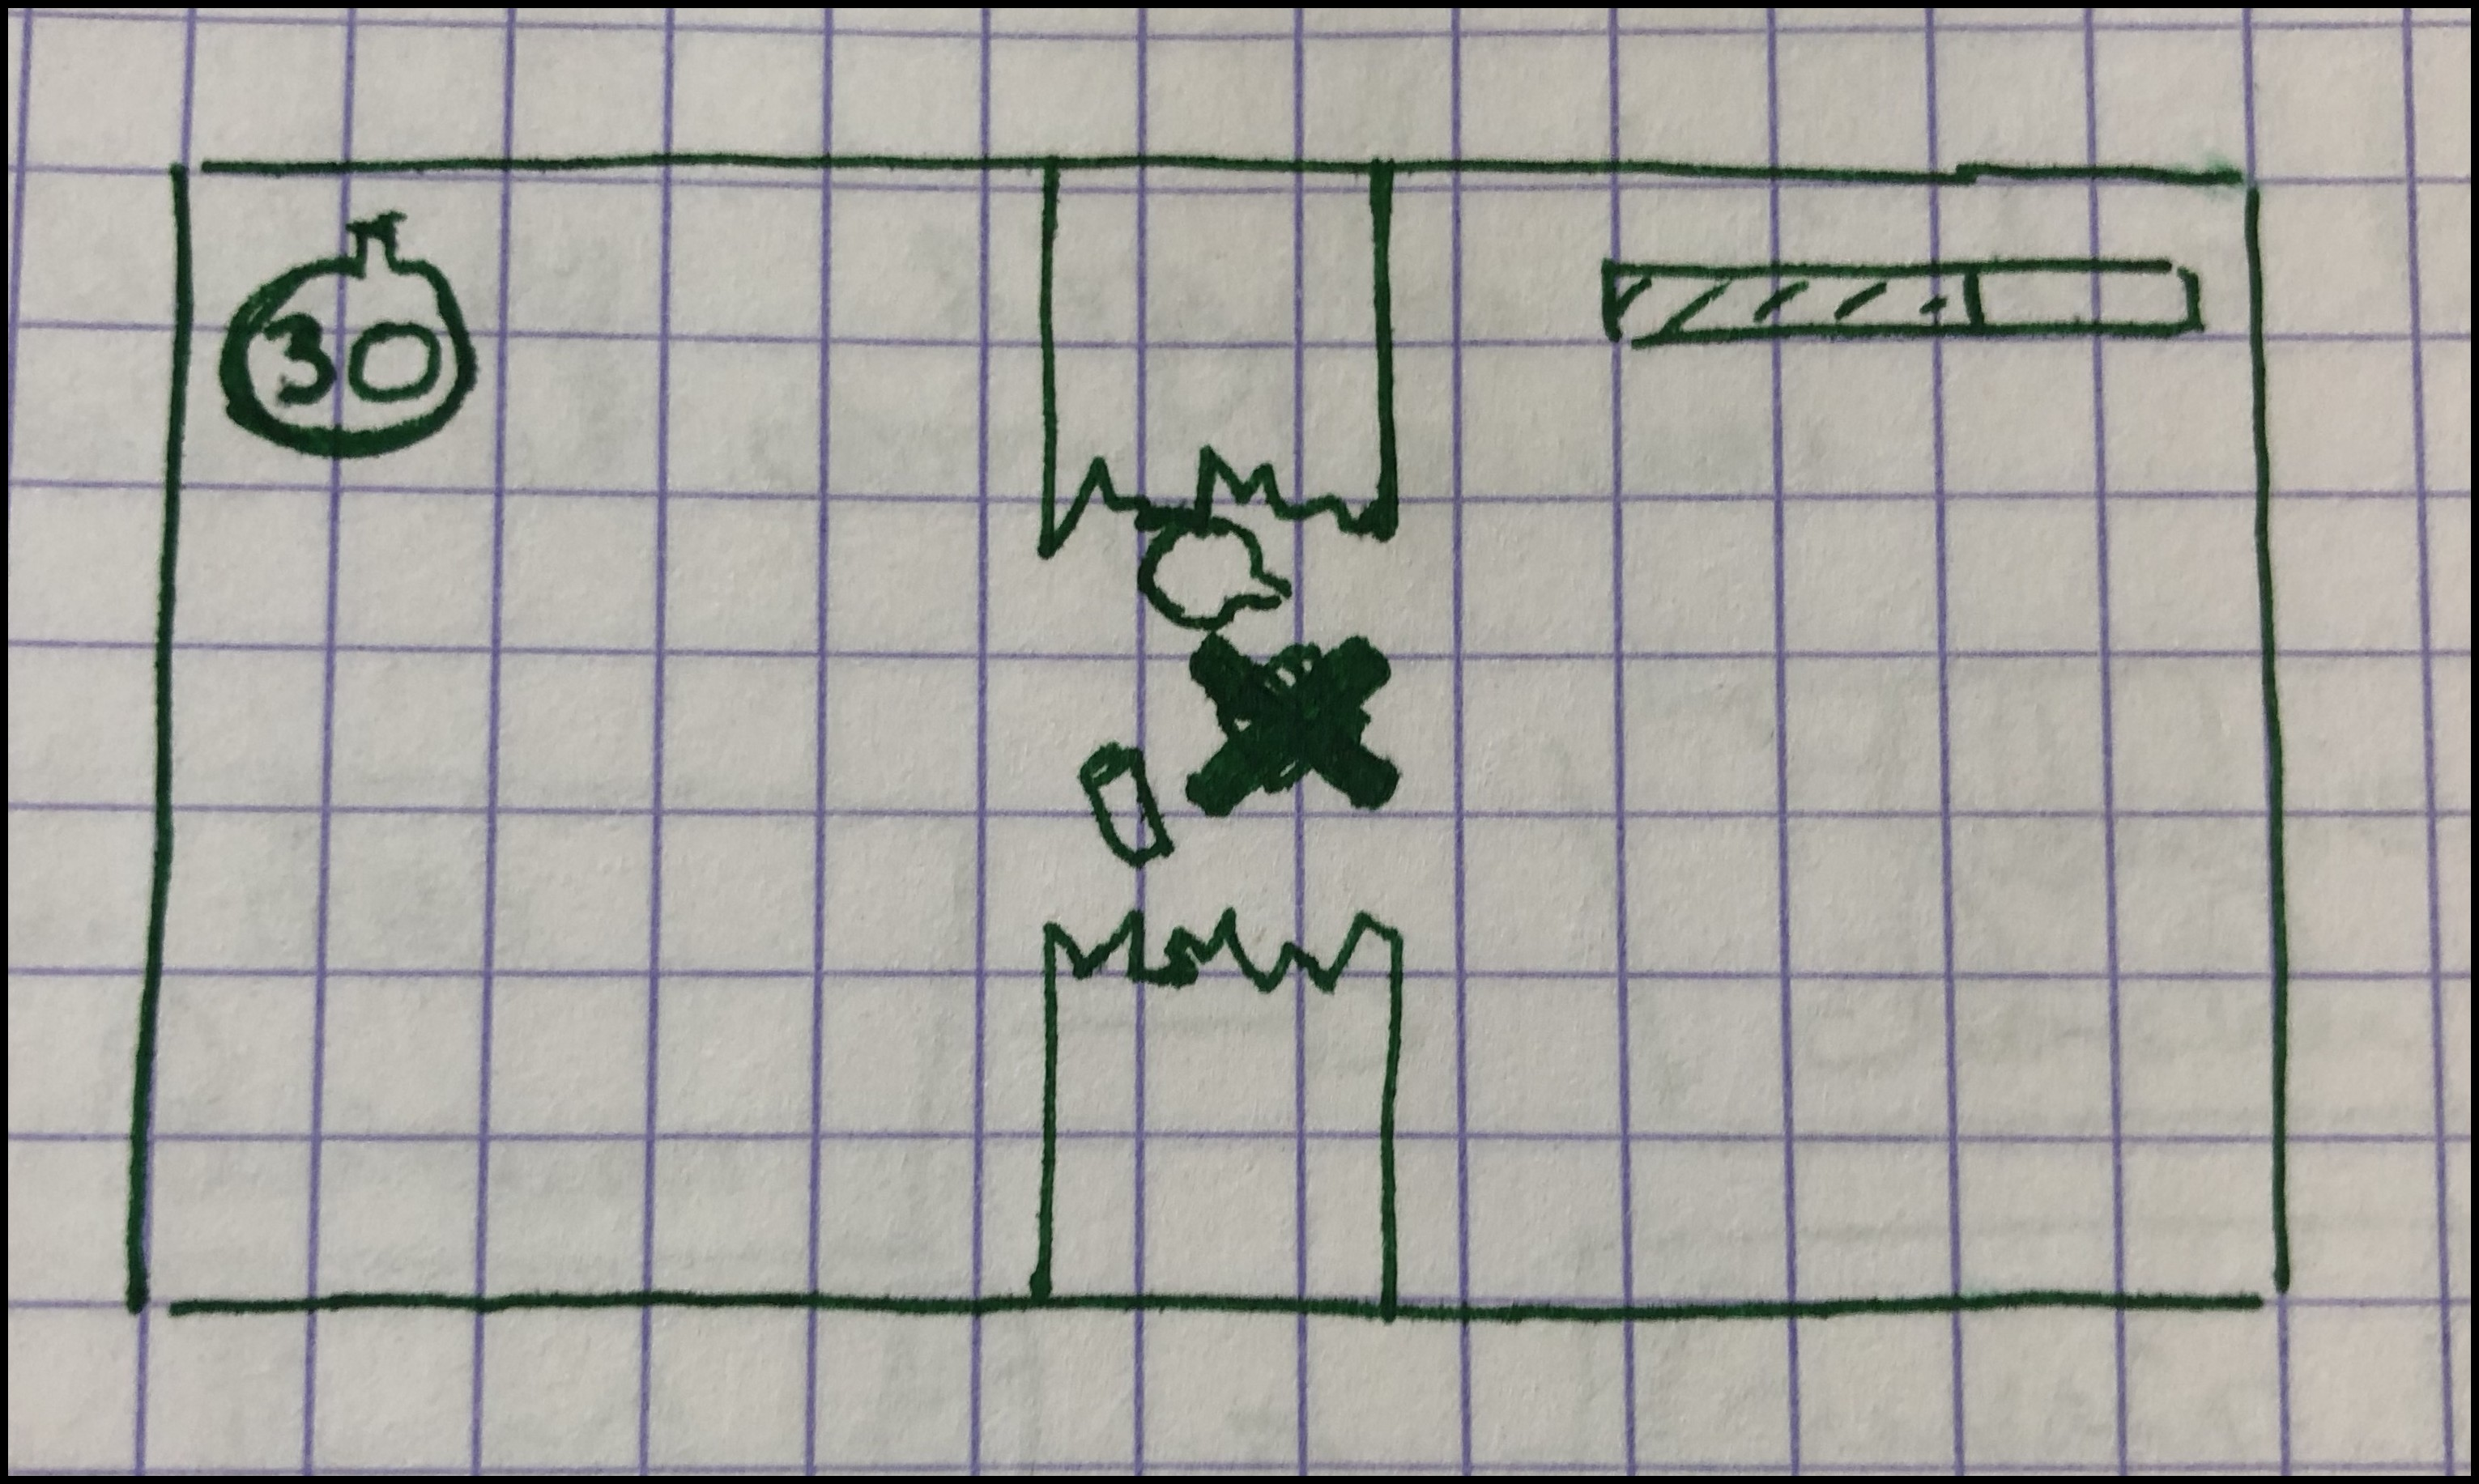
\includegraphics[width=6cm]{miniPipeConcept.jpg}
    \end{center}
    \captionsetup{labelformat=simpleNumber}
    \caption{Concept mini pipe}
\label{MiniPipeConcept}
\end{wrapfigure}

\paragraph{Mini pipe}Le mini jeu du tube était relativement simple. L'idée est que le joueur incarne un mécanicien qui est confronté à une panne dans la machine de tri des matériaux d'un
entrepôt. Il doit alors enlever les matériaux dangereux à la main le temps que les technicien réparent la panne. Le joueur doit donc reconnaitre très rapidement les matériaux qui
défilent pour retirer le bon. Cette mécanique assez proche de la tâche de CPT nous plaisant, nous avons décidé de la pousser plus loin pour en faire notre premier prototype. Mais nous
en parlerons plus en détail dans la partie \ref{prototypage}.

\begin{wrapfigure}[11]{l}{6cm}
    \vspace{-25pt}
    \begin{center}
    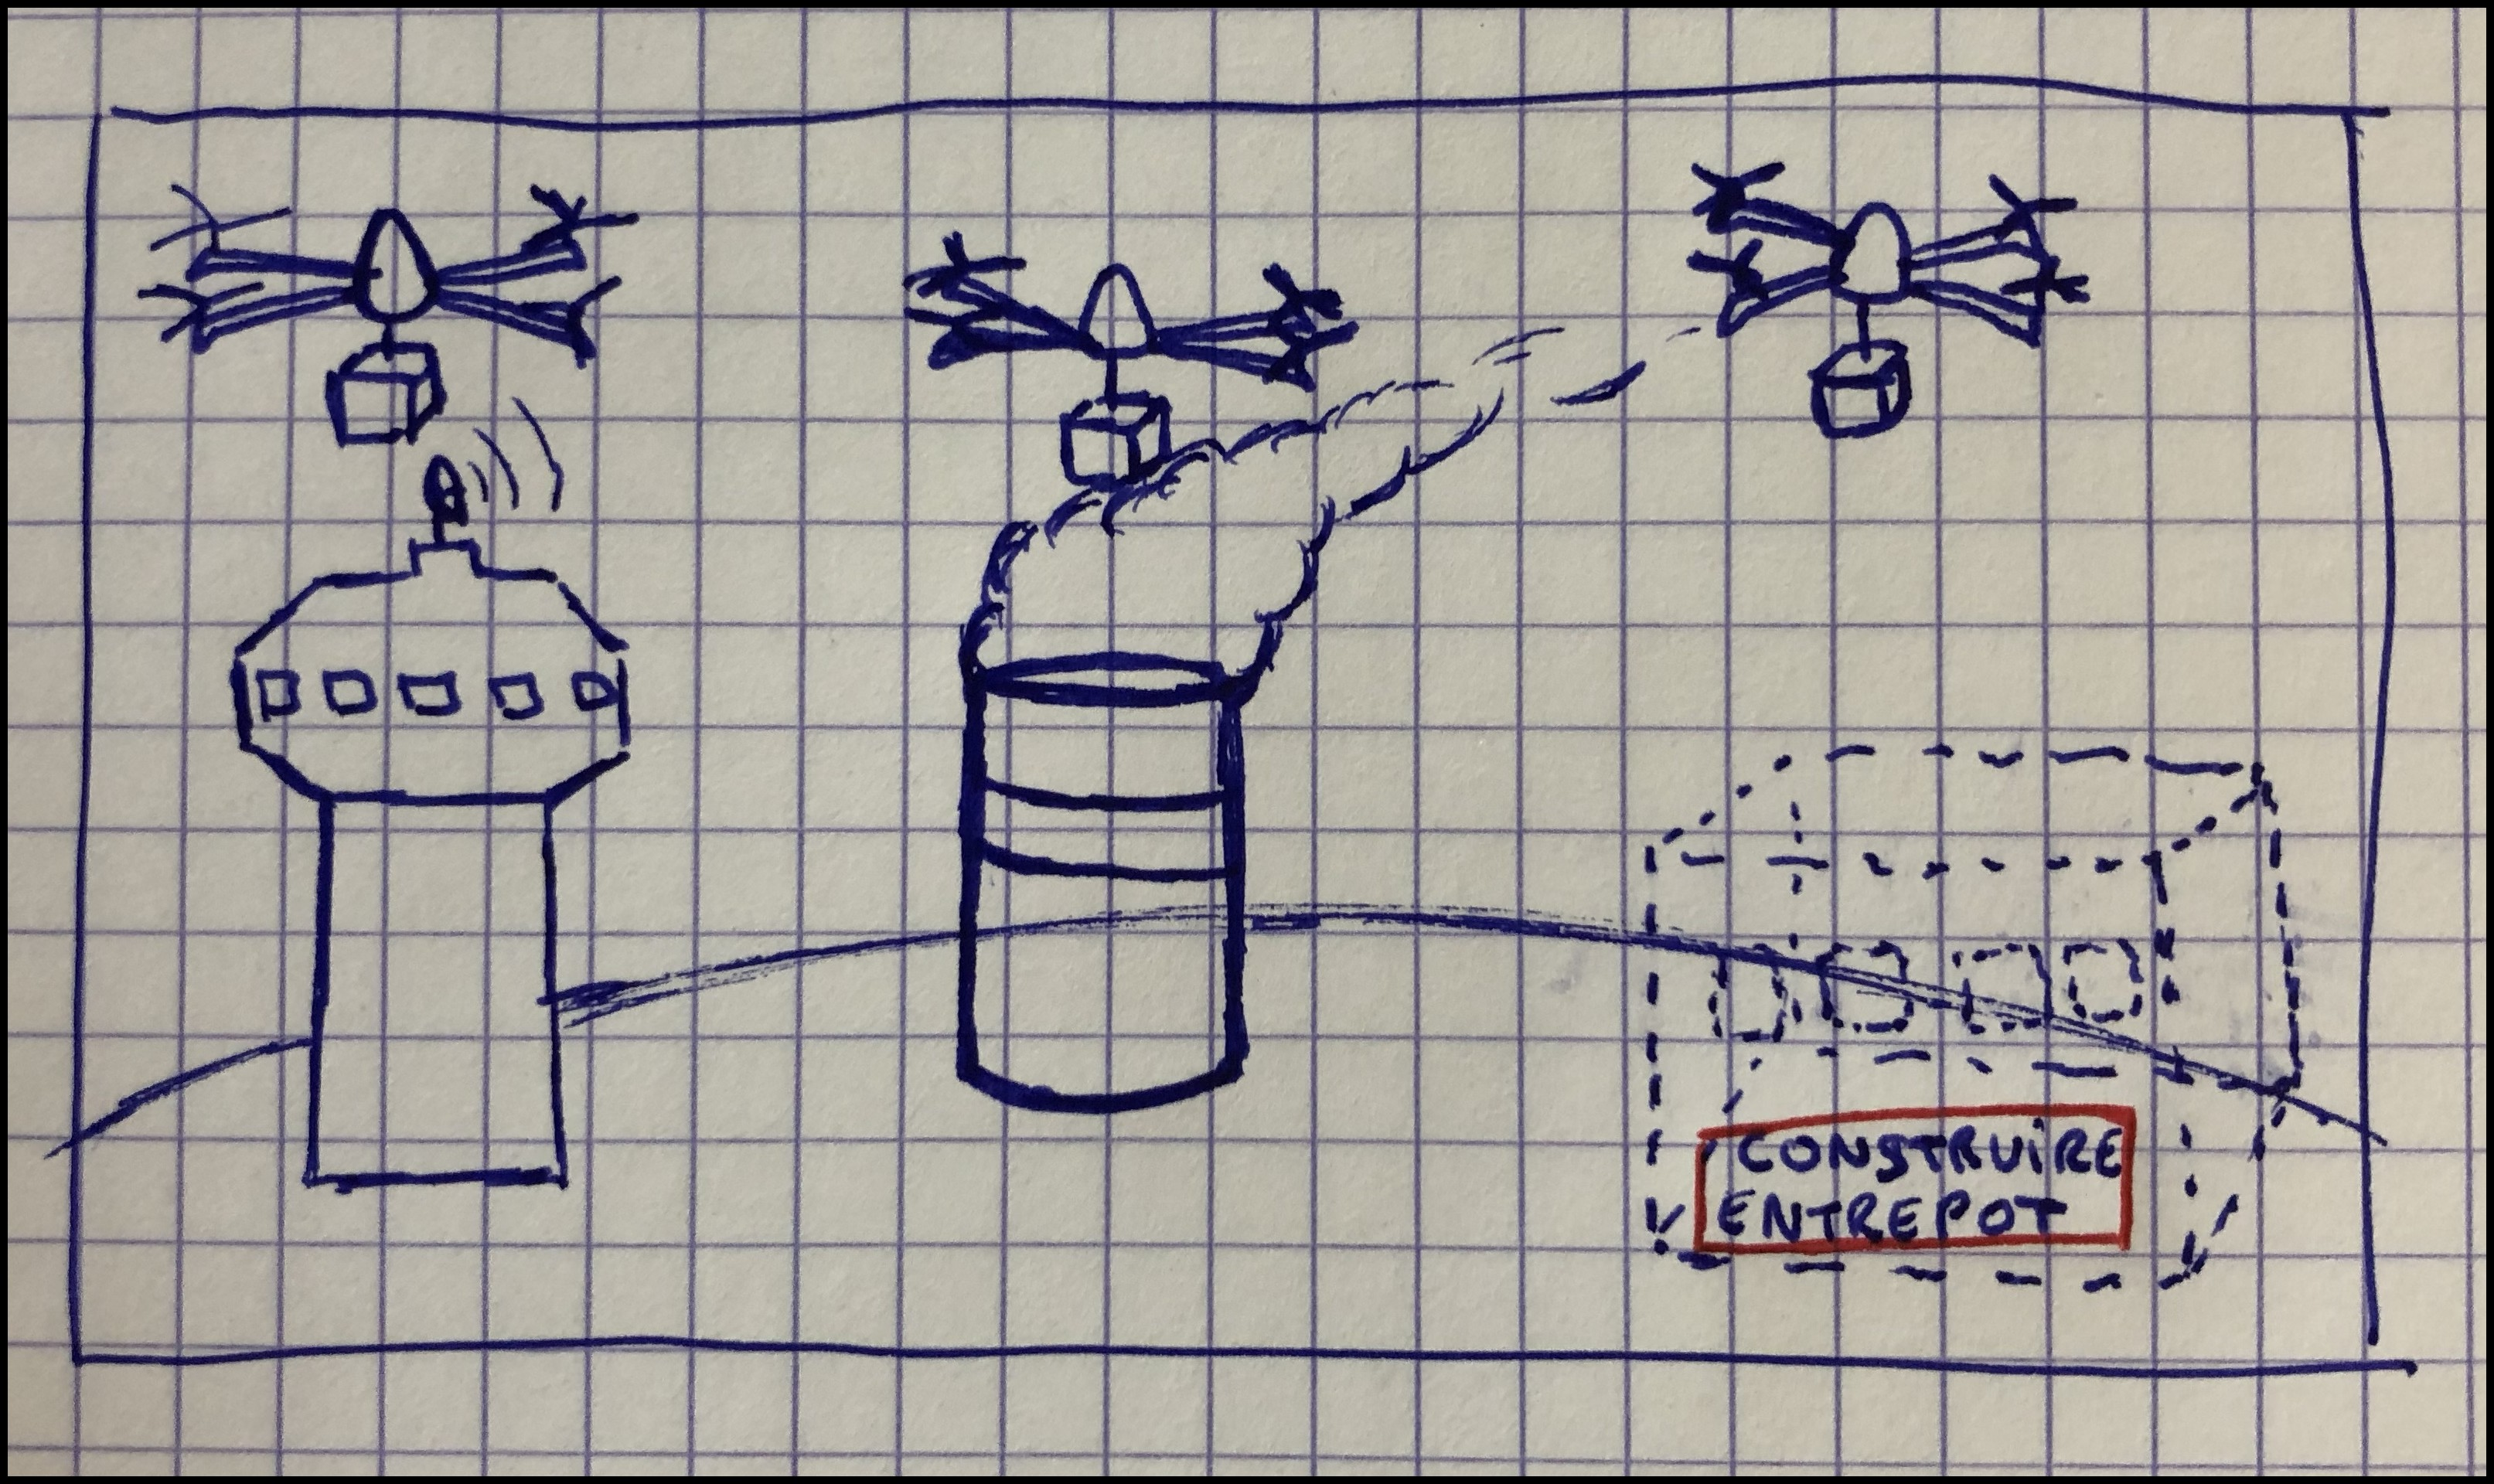
\includegraphics[width=6cm]{drones.jpg}
    \end{center}
    \captionsetup{labelformat=simpleNumber}
    \caption{Mini jeu drones}
\label{Drones}
\end{wrapfigure}

\paragraph{Les drones (anciennement Asterix)} Pour coller au thème de la \gls{SF}, les romains sont devenus des drones. Dans un premier temps, nous avons pensé à envoyer des matériaux
au bons drones. Puis, pour complexifier le mini jeu, nous avons rajouté des éléments de gameplay. Tel un architecte, le joueur doit au contraire récupérer les matériaux dont
il a besoin aux drones correspondant. Le joueur doit avec les matériaux construire les bâtiments d'une base scientifique. Chaque bâtiment nécessite certains matériaux et rapporte un
nombre de points de score défini. Il pourra éventuellement améliorer les bâtiments. Ceux-ci joueront également un rôle dans l'apparition des matériaux. Il devra donc porter son
attention sur plusieurs choses à la fois : les drones qui passent et la construction des bâtiments.

\newpage

\begin{wrapfigure}[17]{l}{6cm}
    \vspace{-10pt}
    \begin{center}
    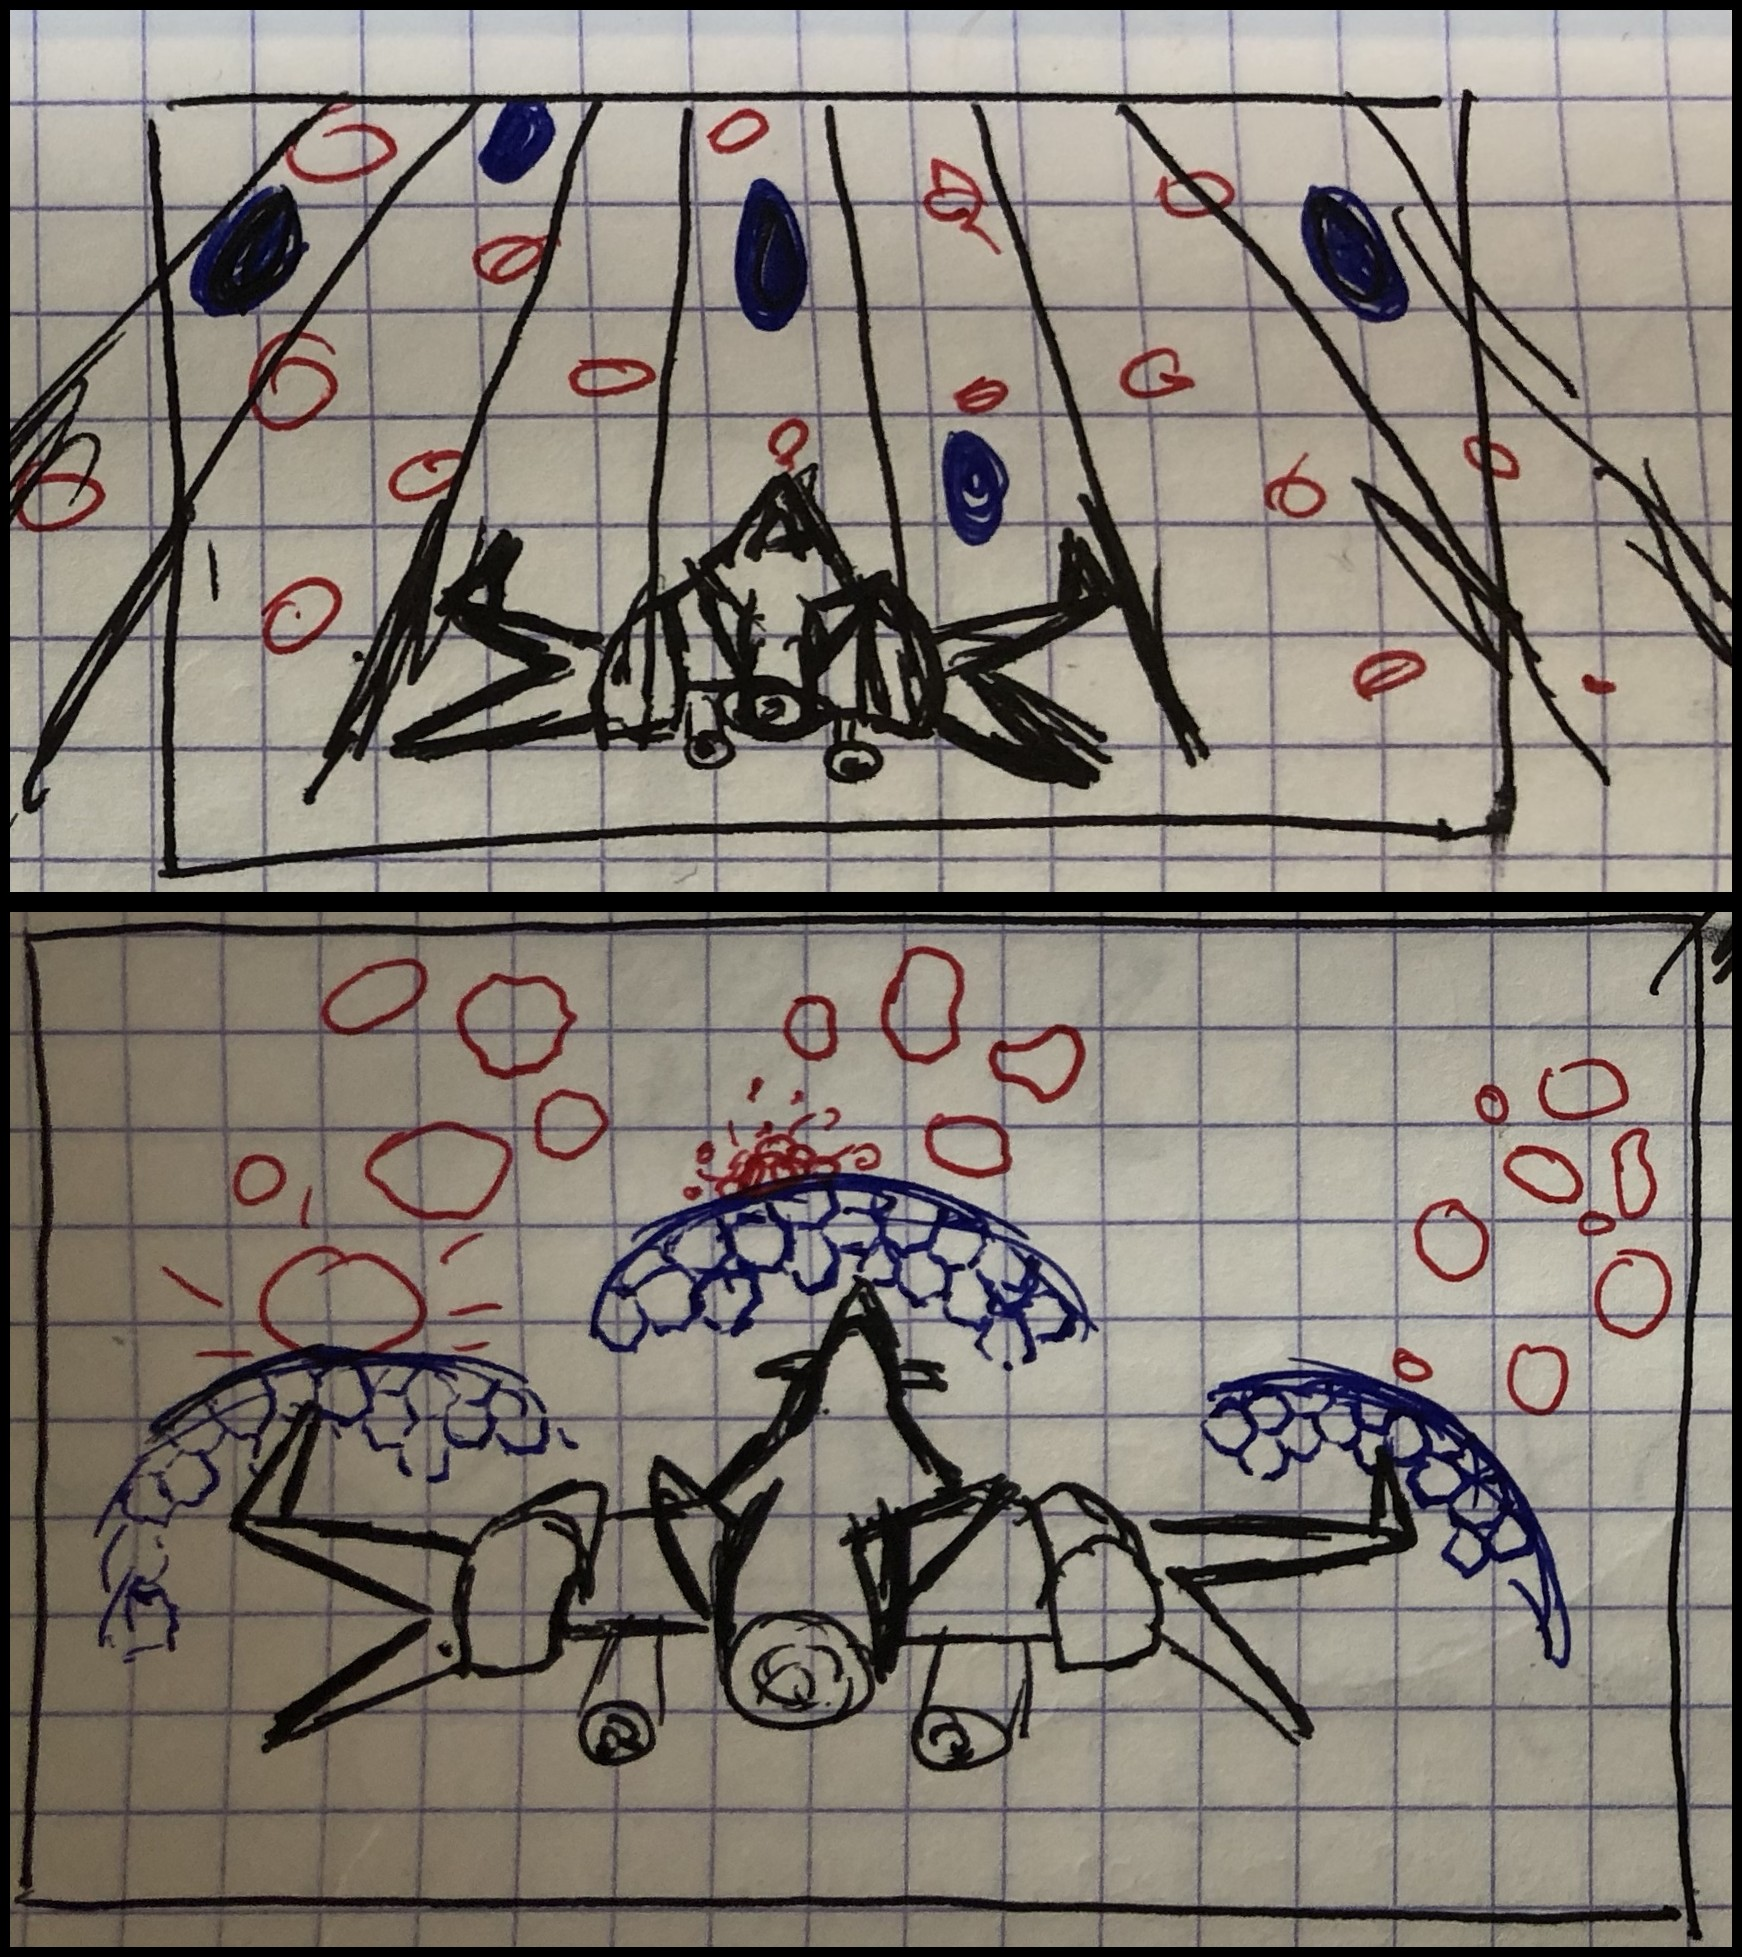
\includegraphics[width=6cm]{spaceship.jpg}
    \end{center}
    \captionsetup{labelformat=simpleNumber}
    \caption{Mini jeu Spaceship}
\label{Spaceship}
\end{wrapfigure}

\paragraph{Spaceship (anciennement Runner)}Le joueur contrôle un vaisseau spatial qui parcourt l'univers. Sur sa route, il croise des météores à éviter qui causent des dommages au
vaisseau, et des naufragés dans des capsules de secours à secourir. Il peut se déplacer à droite ou à gauche pour éviter les météores et dispose d'une recharge de bouclier qu'il peut
placer soit sur l'avant du vaisseau, soit à droite, soit à gauche. Ce bouclier est à utiliser avec parcimonie car il empêche la récupération des naufragés. On peut imaginer une
compétence spéciale qui se recharge au cours du temps, ou au fur et à mesure que le joueur récupère des naufragés. Elle pourrait permettre de détruire tous les météores affichés en
envoyant des missiles téléguidés.


\newpage
\subsubsection{Contexte}

\paragraph{Les mondes}Une des premières discussions concernant le jeu a mis en avant l'importance de faire évoluer le jeu de manière a entrainer petit à petit le joueur a chaque aspect
de l'attention. En effet, le joueur doit d'abord pouvoir se concentrer dans la durée sur un point central fixe. Quand il y arrive, on peut essayer de faire bouger son attention dans
l'espace ... Nous en avons conclu qu'il fallait un "monde" par aspect de l'attention à entrainer. Quatre aspects ont été retenus comme mondes :
\begin{itemize}
\item l'attention soutenue
\item l'attention sélective
\item l'attention divisive
\item l'attention exécutive
\end{itemize}

\paragraph{}Chaque monde possède des niveaux. Ce sont des profondeurs de monde qui permettent d'augmenter la difficulté de manière progressive et montre au joueur sa progression.
Pour débloquer un monde, le joueur doit réussir un certain niveau du monde précédent. Par exemple, si on choisit 7 niveaux par mondes, le joueur doit réussi le niveau 4 du monde 1
pour débloquer le monde 2.

\begin{figure}[H]
    \begin{center}
    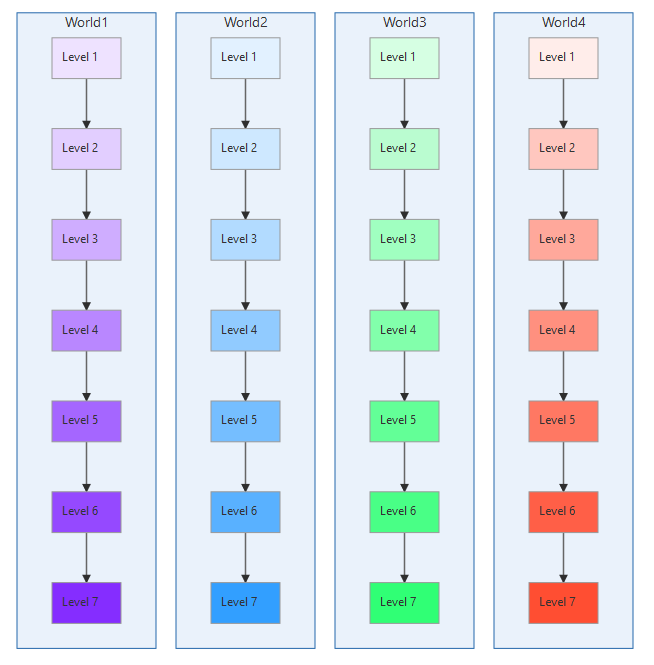
\includegraphics[width=10cm]{profondeurMondes.png}
    \end{center}
    \caption{Profondeur des mondes}
\label{ProfondeurMondes}
\end{figure}

\subsubsection{Le multijoueur}Nous avons d'abord réfléchi au mode multijoueur, bien que celui-ci ne soit développé que dans un second temps après le mode solo. En effet, le mode multi
étant assez important, il nous paraissait logique de penser d'abord à celui-ci pour qu'il y ait de la \emph{cohérence entre le mode solo et le mode multi}. L'idée de ce mode était de
faire collaborer des petits groupes de 4 ou 5 joueurs dans la réalisation d'un but, mais chacun avec ses propres capacités.

En discutant du contexte, nous en sommes venu à la
conclusion qu'il serait intéressant que chaque joueur incarne un personnage différent qui aurait une tâche, un mini-jeu bien précis à faire. La difficulté de celui-ci serait adapté
au joueur. De plus, les meilleurs du groupe sur leur tâche pourraient aider les moins bons grâce à des objectifs secondaires dans leur mini jeu. Lorsque tous réussissent leur tâche,
ils gagnent la partie. On peut aussi penser à mettre en compétition ces groupes entre eux pour créer de l'émulation.

\paragraph{}Il ne faut également pas oublier d'intégrer le professeur dans la boucle de gameplay. Cette partie est à ne pas négliger car le professeur est la personne qui va encadrer les
entrainements des élèves sur le jeu. Il pourrait par exemple créer l'objectif d'une équipe et assigner une tâche à chaque élève, un peu comme un chef d'équipe qui distribue le travail
a son équipe. Il pourrait aussi être celui qui activerait les objectifs bonus dans les tâches des élèves qu'il trouverait performant sur leur tâche pour aider ceux qui auraient plus de
difficultés.

Attention toutefois à ne pas confondre la performance d'un élève sur une tâche et sa performance globale. Un élève peut être performant globalement, avoir des tâches
difficiles, et un jour où il n'est pas très en forme, ne pas être performant sur la tâche. A l'inverse un élève qui n'est pas très performant globalement, en ayant des tâches plutôt
faciles, peut s'il est très en forme réussir haut la main sa tâche. Cet élève-là pourrait alors aider l'élève précédent avec un objectif bonus.

\newpage
\paragraph{Les scénarios}En discutant du multijoueur, l'idée des différents personnages nous a parut très intéressant pour le mode solo : avec des scénarios de personnages différents
dans des contextes différents, on crée de la \emph{généralité}. L'idée était de faire des mini jeux qui paraissent suffisamment différents par leur contexte mais dans lesquels on
demande au joueur de faire appel à leur attention de manière semblable. Ainsi, chaque scénario de personnage pourrait se faire en parallèle des autres, le monde 1 de chaque scénario
correspondant à la même mise en œuvre de l'attention, et cela pour tous les mondes. 

\begin{wrapfigure}[11]{l}{6cm}
    \vspace{-25pt}
    \begin{center}
    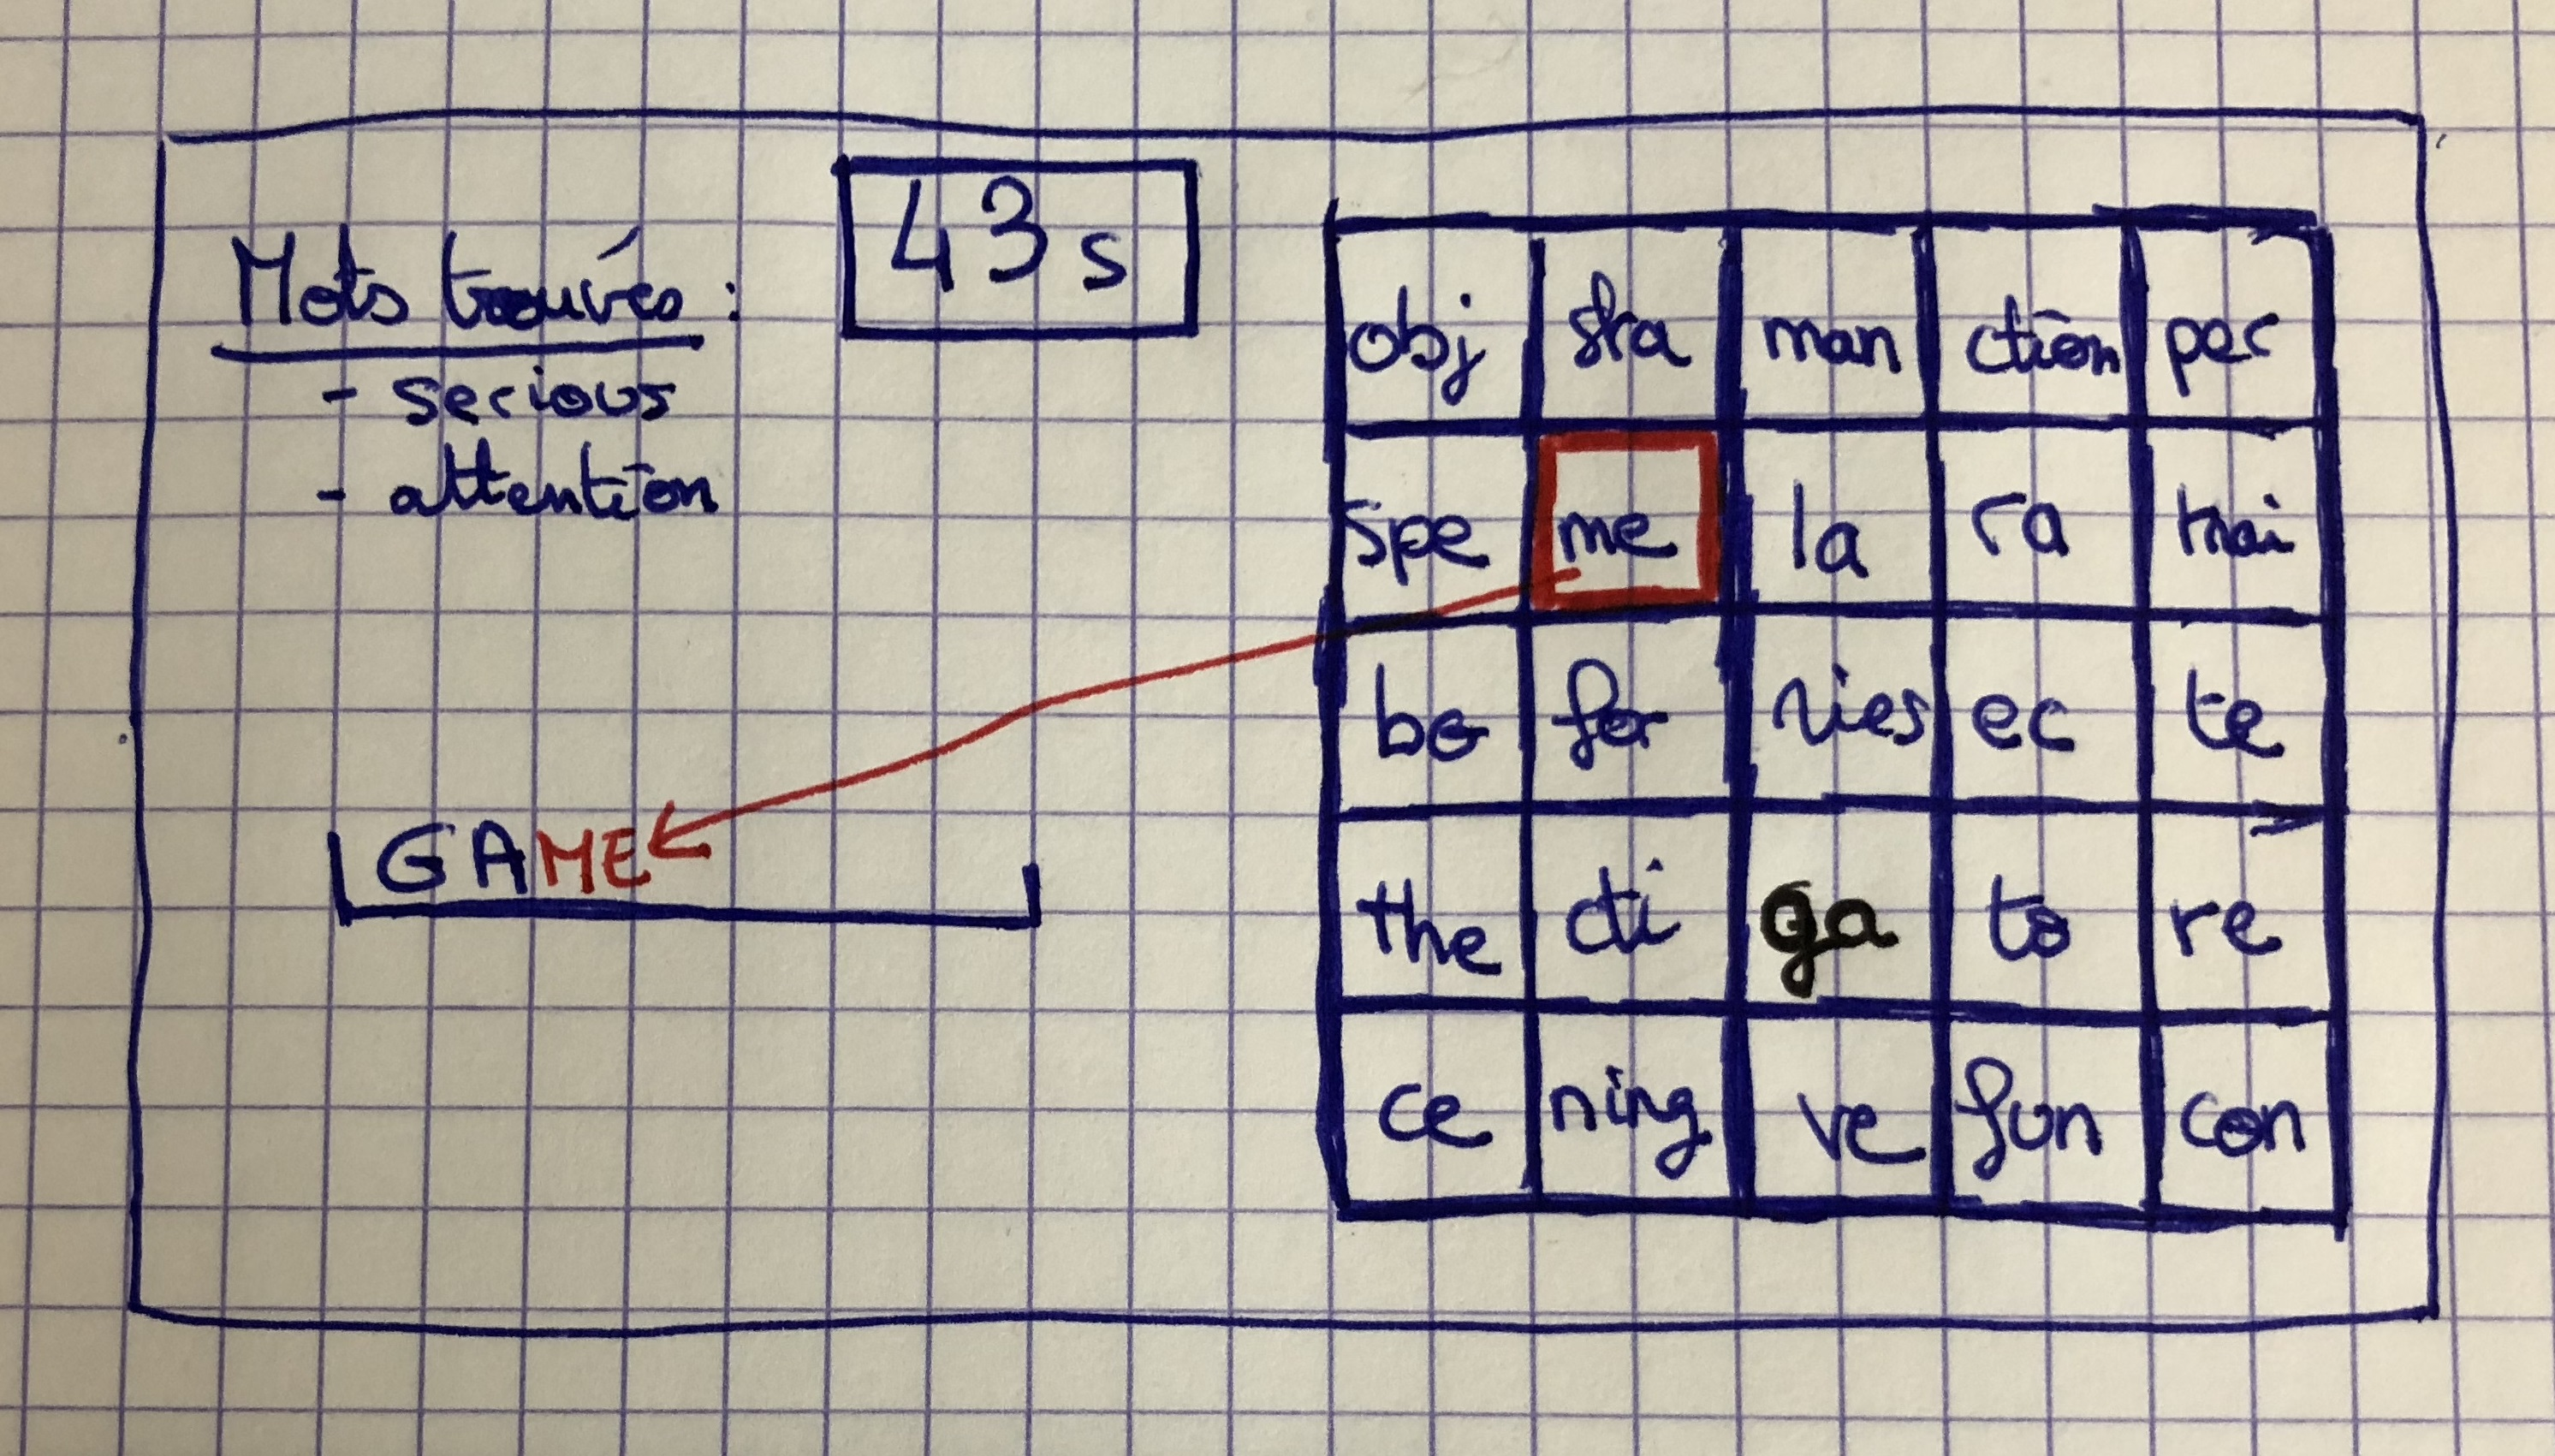
\includegraphics[width=6cm]{hackerConcept.jpg}
    \end{center}
    \captionsetup{labelformat=simpleNumber}
    \caption{Mini jeu Hacker}
\label{Hacker}
\end{wrapfigure}

Nous avons aussi eu l'idée de rattacher les matières étudiées en cours aux mini jeux afin de faire un lien avec l'école dans le jeu. Pour cela, nous avons décidé de relier chaque
personnage à une matière. Le technicien pourrait avoir un lien avec la physique par exemple, le médecin avec la SVT, l'ingénieur avec les mathématiques ou encore le hacker avec des
langues. Un exemple avec le hacker : le joueur doit tester des possibilités de mots de code pour déverrouiller l'accès à un réseau informatique. Il dispose d'une grille de syllabes et
doit reconstituer des mots en anglais. Pour rajouter de la difficulté, les syllabes dans la grille ne restent que 10 secondes, puis sont remplacées de manière désynchronisée par
d'autres.

\begin{figure}[H]
    \begin{center}
    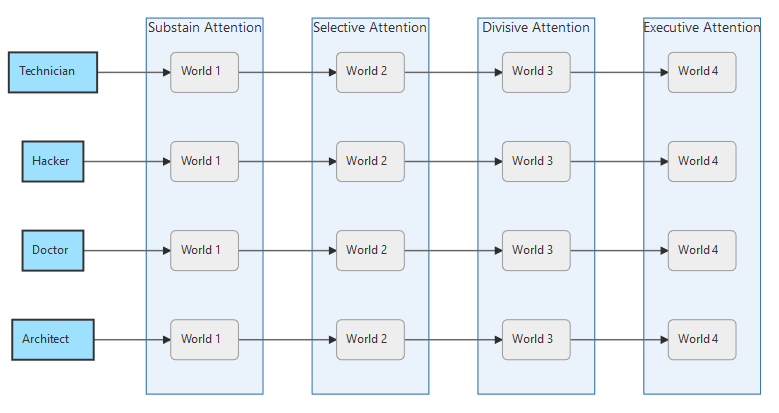
\includegraphics[width=13cm]{scenarios.png}
    \end{center}
    \caption{Scénarios}
\label{Scenarios}
\end{figure}